\section{Evaluation}
\label{sec:eval}

We evaluate our pacing and consumption primitives in three stages: (1)~host-side pacing recovery against unpaced direct push and host-memory DMA rings (\S\ref{sec:eval_pacing}); (2)~a three-way head-to-head comparison of device consumption regimes (\S\ref{sec:eval_rx}); and (3)~end-to-end dual-host 100\,GbE performance on both a lightweight KV store and unmodified upstream Memcached~1.6.45 (\S\ref{sec:eval_e2e}).

\subsection{Host Pacing Recovery}
\label{sec:eval_pacing}

\begin{figure*}[t]
  \centering
  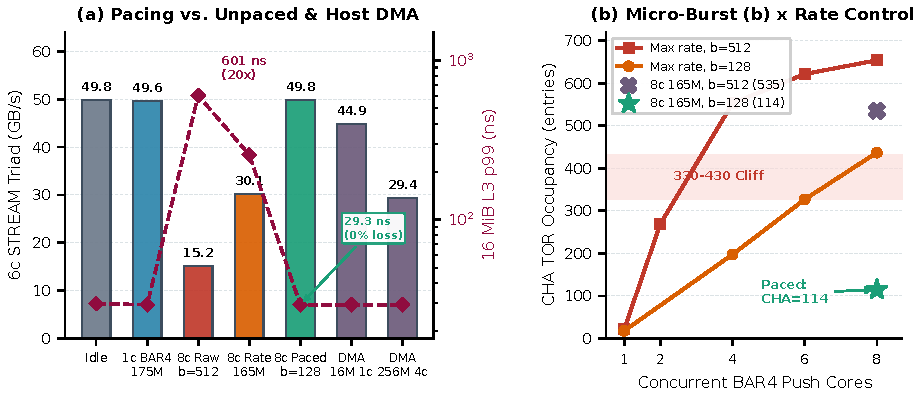
\includegraphics[width=\textwidth]{figures/fig4_pacing_recovery.pdf}
  \caption{Host pacing recovery on CN106 \texttt{BAR4} (516 interleaved runs). (a)~Unpaced 8-core push (\texttt{b=512}) slashes 6-core STREAM Triad by $-$69.5\% and inflates 16\,MiB L3 \texttt{p99} by 20$\times$; aggregate rate capping alone (\texttt{165M, b=512}) still loses $-$39.5\% STREAM and 8.6$\times$ L3 \texttt{p99}. Coupling rate pacing with bounded micro-bursts (\texttt{165M, b=128}) restores 0.0\% neighbor degradation at 94\% of link ceiling, outperforming host-memory DMA rings ($-$9.9\% to $-$41.0\%). (b)~Micro-burst step (\texttt{b=128} vs. \texttt{b=512}) and rate control phase diagram for \texttt{CHA TOR} occupancy.}
  \label{fig:pacing}
\end{figure*}

\autoref{fig:pacing} demonstrates why both rate and micro-burst pacing are essential on CN106 \texttt{BAR4}. At 8 concurrent host cores running unpaced (\texttt{175.5\,Mpps, b=512}), \texttt{CHA TOR} fills to 654.1 entries, collapsing co-located 6-core STREAM Triad from 49.76 to 15.17\,GB/s ($-$69.5\%), spiking 16\,MiB L3 \texttt{p99} from 29.75 to 601.25\,ns (20.2$\times$), and raising 256\,MiB DRAM \texttt{p99} from 135.0 to 1,091.0\,ns (8.1$\times$).

Controlling only one dimension fails to eliminate interference:
\begin{itemize}
  \item \textbf{Aggregate rate pacing alone (\texttt{165.1\,Mpps, b=512}):} Despite staying 10.4\,Mpps below the PCIe Gen5\,$\times$4 ceiling, synchronized 512-line bursts across 8 cores still drive \texttt{CHA TOR} to 535.2 entries (\texttt{M2PCIe1} duty 86.7\%), cutting STREAM Triad by $-$39.5\% (30.11\,GB/s) and inflating L3 \texttt{p99} to 255.0\,ns (8.6$\times$).
  \item \textbf{Micro-burst bounding alone (\texttt{Max rate, b=128}):} Reducing \texttt{b} from 512 to 128 shifts the collapse knee rightward (\autoref{fig:pacing}b), keeping 4-core (\texttt{CHA\,=\,197.3}, STREAM 49.60\,GB/s) and 6-core (\texttt{CHA\,=\,326.7}, STREAM 48.53\,GB/s, L3 \texttt{p99\,=\,29.0\,ns}) safe even at maximum rate. At 8 cores, however, unpaced line-rate contention still crosses into the knee (\texttt{CHA\,=\,436.9}, STREAM 39.96\,GB/s, $-$19.7\%).
  \item \textbf{Coupled rate + micro-burst pacing (\texttt{165.1\,Mpps, b=128}):} Combining both constraints slashes \texttt{CHA TOR} occupancy by 5.7$\times$ down to 114.4 entries (\texttt{MaxBox\,=\,3.7}), completely restoring co-located performance: 6-core STREAM Triad returns to 49.78\,GB/s (+0.0\%), 16\,MiB L3 \texttt{p99} returns to 29.25\,ns, and 256\,MiB DRAM \texttt{p99} returns to 134.0\,ns---all while sustaining 94.1\% of the PCIe Gen5\,$\times$4 write ceiling across 8 concurrent host cores. By comparison, pushing 160\,Mpps through a host-memory DMA ring (\texttt{DPI pull}) incurs $-$9.9\% (16\,MiB, 1c) to $-$41.0\% (256\,MiB, 4c) STREAM loss.
\end{itemize}

\para{Hardware portal partitioning hook ($K\,=\,64/N$).}
On the on-die 4\,KiB Intel DSA portal (\texttt{wq2.0}), our characterization (\S\ref{sec:host_law}) predicts that assigning each of $N \in \{16, 24, 31\}$ physical cores a disjoint slice of $K\,=\,64/N$ cache lines will bound socket-wide \texttt{WCiLF} strictly below 64 entries while preserving near-ceiling 143\,Mpps portal throughput and 0\% neighbor degradation without software rate pacing. Direct experimental results for this disjoint-slice evaluation will be reported in this subsection upon completion of our ongoing Socket~1 hardware verification.

\subsection{Receiver Regimes: Three-Way Head-to-Head}
\label{sec:eval_rx}

\begin{table}[t]
  \centering
  \scriptsize
  \setlength{\tabcolsep}{2.7pt}
  \begin{tabular}{@{}lrrrrr@{}}
    \toprule
    \textbf{Receiver Regime} & \textbf{W=1} & \textbf{CL 1H} & \textbf{CL p99} & \textbf{TX 1H} & \textbf{Host} \\
    \textbf{(CN106 BAR4, 64\,B)} & \textbf{(ns)} & \textbf{(M/s)} & \textbf{(\textmu s)} & \textbf{(M/s)} & \textbf{CHA} \\
    \midrule
    Raw \texttt{Normal-WB} ($K$=4) & 905.5 & 13.53 & 19.91 & 104.24 & \textbf{546.2} \\
    \texttt{B-Queue} \texttt{bq\_probe} ($K$=1, W64) & 900.0 & 13.53 & 5.35 & --- & --- \\
    SW Hyst. Pacing ($C$=32, $b$=16) & 904.5 & 23.68 & 14.68 & 43.08 & \textbf{483.0} \\
    \midrule
    Coalesced DB+\texttt{SFENCE} ($K$=1/2) & 1,096.4 & 66.67 & 4.28 & 118.22 & \textbf{7--12} \\
    Coalesced DB+\texttt{SFENCE} ($K$=4) & 1,096.4 & 54.59 & 5.59 & 105.34 & \textbf{6--11} \\
    \midrule
    \texttt{MT\_NORMAL\_NC} sweet ($K$=2/4) & \textbf{900.9} & \textbf{75.75} & \textbf{3.64} & \textbf{160.10} & \textbf{8--28} \\
    \texttt{MT\_NORMAL\_NC} 2H ($K$=4, W512) & --- & \textbf{119.65} & 8.91 & \textbf{174.10} & 158--256 \\
    \texttt{MT\_NORMAL\_NC} misconf. (\texttt{u4}/\texttt{K=8}) & 916.4 & \textbf{16.27} & 16.51 & 119.61 & \textbf{428--521} \\
    \bottomrule
  \end{tabular}
  \caption{Three-way comparison of CN106 receiver consumption regimes (medians across $n\,=\,3$, 0 errors, 100\% non-multiplexed PMU). CL is closed-loop \texttt{W=256} unless noted; TX is one-way wide-window (\texttt{W=6144}). Host \texttt{CHA} reports TX \texttt{WCiLF} occupancy (entries); bold values $>330$ cross the host collapse cliff.}
  \label{tab:rx_head2head}
\end{table}

\autoref{tab:rx_head2head} summarizes our 183-run head-to-head comparison of three receiver architectures on CN106 \texttt{BAR4} (supplemented by our 633-run \texttt{B-Queue} and open-loop doorbell study):

\para{Software hysteresis pacing on \texttt{Normal-WB}.}
Shaping host credit release (\texttt{C\,=\,32, b\,=\,16}) on \texttt{Normal-WB} preserves 904.5\,ns unloaded RTT and lifts closed-loop throughput from 13.53 to 23.68\,Mmsg/s (+75\%), but cannot break the underlying \texttt{Normal-WB} snoop ceiling: one-way paced TX reaches only 43.08\,Mmsg/s while still driving host \texttt{CHA} to 483.0 entries.

\para{Adaptive coalesced decoupled doorbell + \texttt{SFENCE}.}
Isolating producer notifications onto a separate doorbell line (\texttt{db32}/\texttt{db64}/\texttt{db128}) eliminates data-slot snoops completely. With just 1--2 card cores, it achieves 66.67\,Mmsg/s closed-loop (\texttt{p99\,=\,4.28\,\textmu s}) and 105.34--118.22\,Mmsg/s one-way TX while keeping host \texttt{CHA} rock-steady at 6--12 entries regardless of load. Under open-loop 20 and 25\,Mmsg/s Poisson arrivals, it sustains 19.99 / 24.99\,Mmsg/s with \texttt{p99\,=\,2.46--3.39\,\textmu s} (paired with \texttt{C\_line\,=\,64} for 4 card cores to curb L2 hardware prefetcher overshoot). Its sole costs are +195\,ns at \texttt{W\,=\,1} (1,096.4\,ns) and one batch-tail \texttt{SFENCE}.

\para{Standard Linux \texttt{MT\_NORMAL\_NC} (\texttt{0x44}).}
When properly matched to the workload, \texttt{MT\_NORMAL\_NC} dominates every metric simultaneously: 900.9\,ns \texttt{W\,=\,1} RTT, 75.75\,Mmsg/s 1-host closed-loop (\texttt{p99\,=\,3.64\,\textmu s} using \texttt{u1q}, 128-bit \texttt{ldp q} loads to minimize inner-loop instruction cost), 119.65\,Mmsg/s 2-host closed-loop, and 160.10 / 174.10\,Mpps one-way TX (99.0\%--99.4\% of link ceiling) at \texttt{CHA\,=\,28.2} entries (1H) with zero \texttt{SFENCE}. However, \autoref{tab:rx_head2head}'s final row highlights why adaptive receiver pacing is still required: static misconfiguration (\texttt{u4} in closed loop or over-provisioned $K\,=\,8$) drops closed-loop to 16.27--17.96\,Mmsg/s and drives one-way host \texttt{CHA} back up to 428--521 entries. \emph{Evaluation hook:} Single-binary evaluation of our adaptive empty-poll backoff + \texttt{u4\_ldpq} promotion loop---along with direct co-located 6-core STREAM verification confirming zero neighbor impact at $K\,=\,4$ vs. neighbor degradation at $K\,=\,8$---will complete this table once hardware runs conclude.

\subsection{End-to-End \texorpdfstring{100\,GbE}{100 GbE} Applications}
\label{sec:eval_e2e}

\begin{figure*}[t]
  \centering
  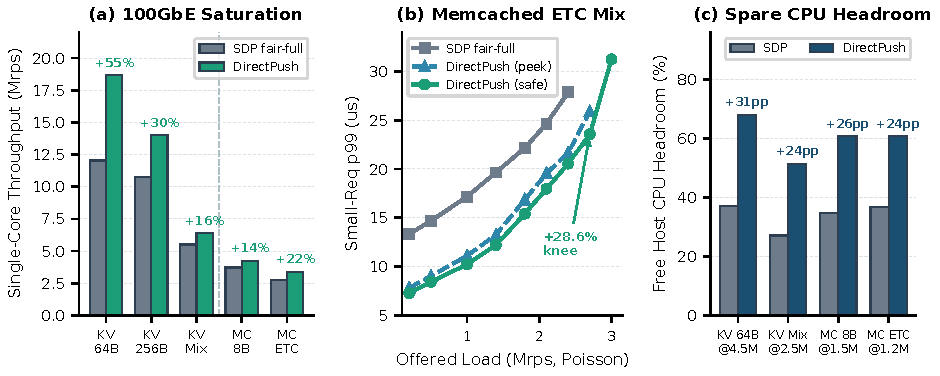
\includegraphics[width=\textwidth]{figures/fig5_e2e_apps.pdf}
  \caption{End-to-end dual-host 100\,GbE evaluation on an in-memory KV store (\texttt{KV}, 453 runs) and zero-modification upstream Memcached~1.6.45 (\texttt{MC}, 406 runs) comparing tuned 4-queue asynchronous \texttt{SDP fair-full} against paced \texttt{DirectPush}. (a)~Single-core saturation throughput (Zipf $s\,=\,0.99$): +55\% on \texttt{KV 64\,B}, +30\% on \texttt{KV 256\,B}, and +22.5\% on \texttt{Memcached} Facebook ETC. (b)~Open-loop Poisson small-request \texttt{p99} latency on \texttt{Memcached} ETC: +28.6\% higher lossless knee (2.10\,$\to$\,2.70\,Mrps). (c)~Matched-rate free host CPU headroom measured via co-running calibrated work units.}
  \label{fig:e2e}
\end{figure*}

To evaluate whether paced MMIO direct push translates into real system-level gains once full RPC parsing, hash-table lookup, locking, and 100\,GbE wire framing are included, we built a paced \texttt{DirectPush} datapath (small responses $\le$\,256\,B pushed via \texttt{BAR4} \texttt{MOVDIR64B} with bounded credits; large 3.8--4\,KiB responses offloaded via \texttt{OP\_DMA} from an LLC-resident 4\,MiB pool; card-to-host RX via write-combining rings) and compared it head-to-head against a heavily tuned 4-queue asynchronous DPDK \texttt{SDP fair-full} baseline (\texttt{4Q\,$\times$\,rxd=512, pool=5119, rx\_poll\_mem=1, tail=48}) across two servers over 100\,GbE (\texttt{saturn} 1 core \texttt{cpu40} @ 3.89\,GHz $\leftrightarrow$ 4-core CN106 $\leftrightarrow$ \texttt{mercury} load generator).

\para{Lightweight in-memory KV store (453 runs).}
Our first server executes a lock-free open-addressing hash table (32.5\,MiB: 16,384 buckets, 8,192 keys, full end-to-end 32-bit checksum and tear validation) with both \texttt{SDP fair-full} and \texttt{DirectPush} sharing identical application code. Under Zipf ($s\,=\,0.99$) traffic (\autoref{fig:e2e}a):
\begin{itemize}
  \item \textbf{Small-request saturation \& tail latency:} On 64\,B GET/PUT, \texttt{DirectPush} increases single-core saturation throughput by +55.1\% (12.04\,$\to$\,18.67\,Mrps with card-side \texttt{direct\_safe}; 17.35\,Mrps, +44.1\% with \texttt{direct\_peek}), constrained by CN106's 4-core forwarding ceiling. At 7.5\,Mrps open-loop Poisson, end-to-end \texttt{p99} falls $-$63.5\% (24.35\,$\to$\,8.89\,\textmu s). On 256\,B GET, saturation rises +30.0\% (10.78\,$\to$\,14.01\,Mrps).
  \item \textbf{Mixed workload isolation:} On a mixed workload (40\% 64\,B, 40\% 256\,B, 20\% 4\,KiB; 84\% GET / 16\% PUT), small/large path separation expands the lossless open-loop knee by +51\% (3.5\,$\to$\,5.3\,Mrps) and cuts small-request \texttt{p99} at 3.5\,Mrps by $-$49.6\% (32.05\,$\to$\,16.14\,\textmu s).
  \item \textbf{PCIe and CPU efficiency:} On 64\,B GET, bidirectional PCIe traffic drops $-$62.5\% (362\,$\to$\,136\,B/RPC, eliminating inbound NIC DMA reads completely: 2.84\,$\to$\,0.00 cache lines/RPC), and matched-rate (4.5\,Mrps) active host CPU falls $-$48.9\% raw (net $-$42.4\% after adjusting for short-quantum empty-poll overhead). On pure 4\,KiB GET/PUT, gains narrow as expected (+3.6\% GET; both hit 99.9\,Gbps wire line rate on PUT), while bypassing DPDK descriptor management still saves 21.4\% raw (15.2\% net) CPU. Two honest boundaries appear: \texttt{direct\_safe} exhibits a 41.9--43.6\,\textmu s tail spike at \texttt{256\,B @ 4.5\,Mrps} Poisson (motivating reverse-order cell publication), and \texttt{4\,KiB @ 1.0\,Mrps} \texttt{p99} is modestly higher than \texttt{SDP} (35.6 vs. 29.6\,\textmu s).
\end{itemize}

\para{Zero-modification upstream Memcached~1.6.45 (406 runs).}
To test whether direct push still pays off inside a heavyweight production engine, we linked all 28 core \texttt{.c} translation units of unmodified upstream Memcached~1.6.45~\cite{memcached2025} (\texttt{git diff\,=\,0} lines across protocol parsing, \texttt{MurmurHash3}, 256\,MiB slab allocator, segmented HOT/WARM/COLD LRU with background maintainer on \texttt{cpu44}, and real \texttt{pthread\_mutex} locks---5 locks per GET, $\ge$8 per SET) via a symmetric 359-line transport adapter.

Under the Facebook ETC Zipf ($s\,=\,0.99$) key-value mix~\cite{atikoglu2012memcached} (\autoref{fig:e2e}a--\ref{fig:e2e}c):
\begin{itemize}
  \item \textbf{Throughput and open-loop latency:} Single-core saturation rises +22.5\% (2.77\,$\to$\,3.39\,Mrps; +20.3\% at 3.33\,Mrps for host-only \texttt{direct\_peek}), and the lossless Poisson knee shifts right by +28.6\% (2.10\,$\to$\,2.70\,Mrps). At 1.40\,Mrps, median latency drops $-$45.9\% (12.72\,$\to$\,6.88\,\textmu s) and small-request \texttt{p99} drops $-$37.8\% (19.64\,$\to$\,12.21\,\textmu s). On pure 8\,B GET, saturation increases +13.9\% (3.72\,$\to$\,4.23\,Mrps; +8.9\% \texttt{direct\_peek}).
  \item \textbf{Spare CPU, PCIe, and DRAM savings:} At matched rates (1.2\,Mrps ETC, 1.5\,Mrps 8\,B GET, 0.6\,Mrps 3.8\,KiB GET), raw co-running work headroom increases by +22.3--26.0\,pp (\autoref{fig:e2e}c); conservatively deducting short-quantum empty-poll overhead yields +10.1--17.5\,pp net spare CPU ($-$27.2\% to $-$32.2\% net active host cycles). Bidirectional PCIe traffic on 8\,B GET falls $-$59.4\% (inbound DMA reads 3.09\,$\to$\,0.00 lines/req), and host DDR5 (\texttt{IMC}) traffic on 3.8\,KiB GET falls 3.1$\times$ at saturation (664.7\,$\to$\,217.4\,B/req, up to 6.2$\times$ in matched open-loop) by avoiding mbuf churn outside the LLC.
  \item \textbf{Amdahl's Law compression:} Consistent with Memcached's heavy core execution (>1,000 cycles/req), pure 3.8\,KiB GET (1.76\,$\to$\,1.79\,Mrps) and lock-heavy 8\,B SET (2.22\,$\to$\,2.17\,Mrps) show minimal throughput change, confirming that transport savings scale strictly with the I/O fraction of CPU time.
\end{itemize}
